% This is LLNCS.DEM the demonstration file of
% the LaTeX macro package from Springer-Verlag
% for Lecture Notes in Computer Science,
% version 2.4 for LaTeX2e as of 16. April 2010
%
\documentclass{llncs}
%
\usepackage{makeidx}  % allows for indexgeneration
\usepackage{llncsdoc}
\usepackage{algorithmic}
\usepackage{amssymb}
\usepackage{graphicx}
\usepackage{wrapfig}
\usepackage{cite}
\usepackage{amsmath}
\usepackage[usenames,dvipsnames]{xcolor}

\newcommand{\Mod}[1]{\ (\text{mod}\ #1)}
\newcommand{\todo}[1]{{\color{red}{TODO #1}}}
%
\begin{document}
\pagestyle{empty}
%
%
\title{TODO}
%
\titlerunning{Research report for UROP course}  % abbreviated title (for running head)
%                                     also used for the TOC unless
%                                     \toctitle is used
%
\subtitle{Undergraduate Research Opportunities}
\author{Drago\c{s} Alin Rotaru}
\authorrunning{D.A.Rotaru} % abbreviated author list (for running head)
%
%%%% list of authors for the TOC (use if author list has to be modified)
%\tocauthor{}

\institute{Universitatea din Bucuresti, Romania\\
\email{r.dragos0@gmail.com
}
}


\maketitle              % typeset the title of the contribution

\begin{abstract}
  None
\keywords{securitate, scheme de partajare}
\end{abstract}

%----------------------------------------------------------------
%----------------------------------------------------------------
%----------------------------------------------------------------
%----------------------------------------------------------------
%----------------------------------------------------------------

\section{Introducere}
\label{sec:intro}

\subsection{Istoric}
Termenul de criptografie este definit in dictionarul Oxford ca fiind "arta de a scrie si a rezolva coduri".
Criptografia moderna s-a desprins de cea clasica in jurul anilor '80, motivand implementarea rigurozitatii matematice pentru definirea constructiilor criptografice. Asta pentru ca in anii anteriori, experienta a dovedit nesiguranta metodelor de criptare, criptanaliza lor fiind uneori triviala (cifrul lui Cezar, Vigenere \ref{wiki:caesar}, \ref{wiki:vigenere}) sau uneori atinsa cu ceva mai mult efort precum Enigma si alte metode din cel de-al doilea razboi mondial. \ref{wiki:enigma}

Criptografia moderna se gaseste pretutindeni in viata de zi cu zi de la ATM-uri, cartele telefonice la semnaturi digitale, protocoale de autentificare, licitatii electronice sau bani digitali, luand amploare o data cu aparitia sistemelor cu cheie publica. O definitie potrivita ar fi "studiul stiintific al tehnicililor pentru a securiza informatia digitala, tranzactiile si calculul distribuit.". \cite{Katz:2007}

\subsection{Motivatie}
\todo{nu are leg\u{a}tur\u{a}: faptul ca sunt scheme cuantice nu are impact asupra structurii de acces; e ok sa men\c{t}ionezi, dar atunci faci asta \^{i}n sec\c{t}iunea anterioar\u{a}, c\^{a}nd po\c{t}i s\u{a} adaugi \c{s}i alte modalit\u{a}\c{t}i de definire: scheme bazate pe latici, scheme bazate pe perechi biliniare, scheme cuantice, etc.}
%TODO: maybe wrap this up in a definition
Dezavantajul schemelor generale de partajare este dimensiunea componentelor, exponentiala in functie de numarul de participanti. \cite{Survey:2011}
De asemenea, s-au dezvoltat scheme pentru modele de calcul neconventional, cum ar fi cel cuantic. \cite{hillery:1999} %maybe expand this
%Poate aici vine mai bine sub sectiunea cu securitatea teoretica

\subsection{Structura}
TODO

%----------------------------------------------------------------
%---------------------------------------------------------------
%----------------------------------------------------------------
%----------------------------------------------------------------
%----------------------------------------------------------------

\subsection{Securitatea Teoretica a Informatiei}

In cazul unor criptosisteme acestea nu pot fi compromise chiar daca adversarul dispune de o putere computationala nelimitata. Cateva exemple de criptosisteme care garanteaza securitatea teoretica-informationala sunt: schemele de partajare, unele protocoale multi-party computation, preluarea intr-un mod sigur(securizat?) informatii de la baze de date. Securitatea teoretica vine insa cu un cost: efortul computational depus este mult mai mare decat in cazul schemelor care nu garanteaza securitatea teoretica (se bazeaza pe dificultatea computationala unor probleme cunoscute). \cite{L:1997}

%----------------------------------------------------------------
%----------------------------------------------------------------
%----------------------------------------------------------------
%----------------------------------------------------------------
%----------------------------------------------------------------
\section{Scheme de partajare}

\label{sec:encryption}
%TODO: find translation for multi party computation

O schema de partajare consta in distribuirea unei informa\c{t}ii secrete $\mathcal{S}$ la mai mul\c{t}i participan\c{t}i astfel \^{i}nc\^{a}t oricare superset de participan\c{t}i predefinit inainte (o structur\u{a} de acces pe care o vom denumi $\mathcal{A}$) sa poat\u{a} reconstitui secretul $\mathcal{S}$.
Formal, o schem\u{a} de partajare este reprezentat\u{a} de o pereche de algoritmi \textbf{$(Gen, Rec)$}:
\begin{itemize}
	\item \textit{$Gen(S, m)$} este un algoritm care prime\c{s}te la intrare un secret \textit{S} \c{s}i un num\u{a}r \^{i}ntreg $m$ \c{s}i \^{i}ntoarce un set de componente ${s_1, s_2, \dots, s_m}$.
	\item \textit{$Rec({s_i}_1, {s_i}_2, \dots, {s_i}_q)$} este un algoritm care prime\c{s}te ca parametri de intrare o mul\c{t}ime de componente si \^{i}ntoarce \textit{S} dac\u{a} mul\c{t}imea ${s_i}_1, {s_i}_2, \dots, {s_i}_q \in \mathcal{A}$.
\end{itemize} 
%todo: add some more text between itemizers
Majoritatea schemelor constau \^{i}n mai multe etape precum:
\begin{itemize}
	\item \textit{Ini\c{t}ializare}. Presupune ini\c{t}ializarea variabilelor de mediu necesare.
	\item \textit{Generare}. O entitate autorizat\u{a} (numit\u{a} dealer) $\mathcal{D}$ folose\c{s}te algoritmul \textit{Gen} pentru a genera componentele.
	\item \textit{Distribu\c{t}ie}. Componentele sunt trimise participan\c{t}ilor cu ajutorul unui mijloc de comunicare sigur, f\u{a}r\u{a} ca acestea sa fie vizibile unui atacator.
	\item \textit{Reconstruc\c{t}ie}. D\^{a}ndu-se o mul\c{t}ime de componente, se folose\c{s}te algoritmul \textit{Rec} pentru a recupera secretul
	$\mathcal{S}$.
\end{itemize}

Acestea se clasific\u{a} in func\c{t}ie de cantitatea de informa\c{t}ie secret\u{a} pe care o pot ob\c{t}ine persoanele care nu fac parte din $\mathcal{A}$ \cite{Martin:2008}:
\begin{itemize}
	\item \textit{Sisteme perfecte de partajare}: componentele nu ofer\u{a} nici o informatie teoretica despre $\mathcal{S}$ indiferent de resursele computa\c{t}ionale.
	\item \textit{Sisteme statistic sigure}: o frac\c{t}iune de informa\c{t}ie este dezvaluita despre $\mathcal{S}$ independent de puterea computionala a adversarului.
	\item \textit{Sisteme computa\c{t}ional-sigure de partajare}: se bazeaz\u{a} pe faptul ca reconstituirea lui $\mathcal{S}$ se reduce la o problema \textit{dificil\u{a}}\cite{boneh:1998decision} in lipsa unor informa\c{t}ii oferite doar grupului de acces $\mathcal{A}$.
%cite somehow AA article \todo{nu toate problemele sunt demonstrate ca fiind NP complete, se crede ca sunt probleme dificile}. ups, forgot about that:)
\end{itemize} 

\^{I}n continuare vom prezenta cateva sisteme perfecte de partajare pentru a forma funda\c{t}iile utilizate de arhitecturi pentru stocarea fisierelor, disponibile pe o durata indelungat\u{a}.

\subsection{Istoric}

Primele scheme de partajare au fost dezvoltate independent de Shamir si Blakley in 1979 \cite{B:1979, S:1979}.

Denumite \c{s}i scheme majoritare $(k, n)$, acestea rezolvau cazul in care oricare grup de participanti cu un num\u{a}r mai mare sau egal dec\^{a}t $k$  (m\u{a}rimea pragului) poate reconstitui secretul $\mathcal{S}$ din componentele primite de la dealer. Dac\u{a} schema este perfect \textit{sigur\u{a}} atunci oricare grup cu un num\u{a}r de participan\c{t}i mai mic decat $k$ nu ob\c{t}ine vreo informa\c{t}ie despre $\mathcal{S}$.

Not\u{a}m $P = \{P_1, \dots, P_n\}$ mul\c{t}imea format\u{a} din cei $n$ participan\c{t}i \^{i}ntr-o schem\u{a} \c{s}i $y \leftarrow^R Y$ ca $y$ este un element ales uniform aleator din mul\c{t}imea $Y$.

Alte scheme de partajare baz\^{a}ndu-se pe structuri de acces generale au fost dezvoltate de Ito, Saito, si Nishizeki, realiz\^{a}nd o generalizare a schemei Shamir. \cite{ITO:1989}
Benaloh si Leichter au demonstrat ca schemele de partajare de tip prag nu pot fi folosite pe structuri general monotone (familie de submul\c{t}imi ale lui $P$) si ob\c{t}in o construc\c{t}ie mai eficient\u{a} ca Ito et. al \cite{ITO:1989} din punct de vedere al num\u{a}rului de componente distribuite participan\c{t}ilor. \cite{JJ:1990}

Autorii prezint\u{a} un exemplu trivial pentru care schema Shamir este insuficient\u{a}. Consider\u{a}m cazul in care vrem sa partajam un secret \^{i}ntre 4 participan\c{t}i: $P_1, P_2, P_3, P_4$ astfel \^{i}nc\^{a}t $\{P_1,P_2\}$ \c{s}i $\{P_3,P_4\}$ s\u{a} fie singurele mul\c{t}imi autorizate pentru reconstruc\c{t}ia secretului $S$ (i.e. $\mathcal{A} = \{ \{P_1,P_2\}, \{P_3,P_4\} \}$).

\subsection{Schema unanim\u{a}}

Presupun\^{a}nd ca vrem sa imp\u{a}r\c{t}im un secret $\mathcal{S}$ la $n$ participan\c{t}i astfel \^{i}nc\^{a}t $\mathcal{S}$ sa poat\u{a} fi recuperat doar daca to\c{t}i cei $n$ participan\c{t}i \^{i}\c{s}i combin\u{a} componentele pe care le de\c{t}in. Metoda este echivalent\u{a} cu o schem\u{a} $(n, n)$ majoritar\u{a}. Un exemplu este schema introdus\u{a} de Karin, Greene \c{s}i Hellman \cite{Karnin:83} (Fig.\label{fig:all_or_nothing})


%---------------- Figure - all_or_nothing - START ------------------------
\begin{figure*}[h!]

\begin{tabular}{|p{\textwidth}|}
\hline

\\
\hspace{.1in}
\textbf{Ini\c{t}ializare}: 
	\begin{itemize}
		\item Fie $S \in Z_q$ unde $q > 1 $ si $q$ prim;
		\item Fie $n$ num\u{a}rul de participan\c{t}i;
	\end{itemize}
\medskip

\hspace{.1in}
\textbf{Generare}: Dealerul $\mathcal{D}$:
	\begin{itemize}
		\setlength{\itemsep}{5pt}
		\item Alege $n - 1$ valori aleatoare $s_i \leftarrow^R Z_p$, $i \in \{1,2,\dots,{n-1}\}$;
		\item $s_n = S + \sum\limits_{i=1}^{n-1} s_i \Mod q $;
	\end{itemize}
\medskip

\hspace{.1in}
\textbf{Distribu\c{t}ie}: Dealerul $\mathcal{D}$
	\begin{itemize}
		\item transmite \^{i}n mod sigur participantului $P_i$ componenta $s_i$, $i \in \{1,2,\dots,n\}$;
	\end{itemize}

\hspace{.1in}
\textbf{Reconstruc\c{t}ie}: Cei $n$ participan\c{t}i:
	\begin{itemize}
		\item Calculeaz\u{a} $S = \sum\limits_{i=1}^{n} s_i \Mod q$.
	\end{itemize}

\\
\hline
\end{tabular}
\caption{Schema unanim\u{a} \cite{Karnin:83}}
\label{fig:all_or_nothing}
\end{figure*}

%---------------- Figure - all_or_nothing- STOP ------------------------



\subsection{Schema Shamir}
%TODO complete description

Schema Shamir ofera mai mult\u{a} flexibilitate ca schema unanima prin faptul ca oricare $k$ (sau mai multi) participan\c{t}i
din cei $n$ pot recupera $\mathcal{S}$, \^{i}ns\u{a} mai pu\c{t}in de $k$ nu ob\c{t}in nicio informa\c{t}ie despre $\mathcal{S}$. Schema Shamir este deci o schem\u{a} $(k,n)$ majoritar\u{a}.

Intuitiv, av\^{a}nd $k$ puncte in plan $(x_i, y_i)$, $x_i \neq x_j \text{ } i,j \in \{1,2,\dots,k\}$ $\forall i \neq j$, exist\^{a} o curb\u{a} polinomial\u{a} unic\u{a} care trece prin ele.  
In schimb, pentru a defini o curb\u{a} polinomial\u{a} de grad $k$ care con\c{t}ine $k - 1$ puncte date, exista o infinitate de solu\c{t}ii.
Evident, orice submul\c{t}ime de valori $s_i$ de m\u{a}rime egal\u{a} cu $k$ este suficient\u{a} \c{s}i necesar\u{a} pentru a reconstrui polinomul $f$. Dupa interpolarea componentelor de\c{t}inute de cel pu\c{t}in $k$ dintre participan\c{t}i, secretul $\mathcal{S}$ se va afla in $f(0)$. (Fig. \ref{fig:shamir_scheme}) 

Pentru un atacator care de\c{t}ine chiar \c{s}i $k-1$ valori $\mathcal{S}_i$, acesta nu determin\u{a} nimic despre $\mathcal{S}$, spa\c{t}iul de solu\c{t}ii posibile fiind identic fa\c{t}\u{a} de situa\c{t}ia in care nu reu\c{s}e\c{s}te sa ob\c{t}in\u{a} vreo component\u{a}.

%---------------- Figure - shamir_scheme - START ------------------------
\begin{figure*}[h!]

\begin{tabular}{|p{\textwidth}|}
\hline

\\
\hspace{.1in}
\textbf{Ini\c{t}ializare}: 
	\begin{itemize}
		\item Fie $S \in Z_q$ unde $q > 1 $ si $q$ prim;
		\item Fie $n$ num\u{a}rul de participan\c{t}i a.i $q > n$;
		\item Fie $k$ num\u{a}rul minim de componente puse in comun pentru a determina pe $\mathcal{S}$;
	\end{itemize}
\medskip

\hspace{.1in}
\textbf{Generare}: Dealerul $\mathcal{D}$:
	\begin{itemize}
		\item Alege $n$ valori distincte $x_i \leftarrow^R Z_q \text{, }i = 1,2,\dots,n$;
		\item Alege $a_{i} \leftarrow^R Z_q \text{, }i \in \{1,2,\dots,{k - 1}$\}, $a_{k-1} \neq 0$;
		\item Construie\c{s}te polinomul $f(x) = a_{k - 1}x ^ {k-1} + a_{k-2}x ^ {k - 2} + \dots + a_1x + \mathcal{S}$;
		\item Calculeaz\u{a} $s_i = f(x_i) \text{ } i \in \{1,2,\dots,n\}$;
	\end{itemize}
\medskip

\hspace{.1in}
\textbf{Distribu\c{t}ie}: Dealerul $\mathcal{D}$:
	\begin{itemize}
		\item Transmite participantului $P_i$ componenta $s_i$, $i \in \{1,\dots,n-1\}$;
	\end{itemize}

\hspace{.1in}
%TODO: aranjeaza cu "(sau mai mare)"
\textbf{Reconstruc\c{t}ie}: Orice mul\c{t}ime cu dimensiunea $k$ (sau mai mare) de participan\c{t}i distinc\c{t}i $P_1, P_2, \dots, P_k$:
	\begin{itemize}
		\setlength{\itemsep}{5pt}
		\item Interpoleaz\u{a} punctele $s_i$ pentru a ob\c{t}ine polinomul $f$:
		\begin{equation} f(x)=\sum_{i=1}^{k} {s_i}\prod_{1 \leq j \leq k, j \neq i} \frac{x-x_j}{x_i-x_j} \end{equation}
		\item Afl\u{a} secretul reconstruit $S = f(0)$.
	\end{itemize}

\\
\hline
\end{tabular}

\caption{Schema Shamir \cite{S:1979}}
\label{fig:shamir_scheme}
\end{figure*}

%---------------- Figure - shamir_scheme- STOP ------------------------

\subsection{Schema Ito, Saito, si Nishizeki}
\label{Ito}

In continuare vom descrie modalitatea de distribuire a componentelor de la care au pornit Ito, Saito si Nishizeki pentru ca schema sa aiba o structur\u{a} de acces $\mathcal{A} \subseteq 2^P$ (submul\c{t}ime a supersetului de participan\c{t}i) a.i $\forall A \in \mathcal{A}, A \subseteq A' \Rightarrow A' \in \mathcal{A}$).
Av\^{a}nd construc\c{t}ia unei scheme majoritare $(k, n)$ autorii au reu\c{s}it s\u{a} descrie elementele din $\mathcal{A}$ folosind rezultatul unei reuniuni de mul\c{t}imi de componente cu un num\u{a}r de elemente mai mare sau egal decat $k$. Definim $x : Pr$, $x$ are proprietatea $Pr$. Fig. \ref{fig:ito_et_al} detaliaz\u{a} construc\c{t}ia.

Dezvantajul acestei structuri este num\u{a}rul de componente necesar pentru o structur\u{a} de acces oarecare $\mathcal{A}$. Un mod simplu de construire al func\c{t}iei $Assign$ este Pentru mai multe informatii despre functia $Assign$, cititorul interesat poate citi in \cite{ITO:1989}.
\todo{prezentarea trebuie s\u{a} fie de sine st\u{a}t\u{a}toare, trebuie m\u{a}car s\u{a} explici \^{i}n cuvinte ce \^{i}nseamn\u{a}}



%---------------- Figure - Ito_et_al- START ------------------------
\begin{figure*}[h!]

\begin{tabular}{|p{\textwidth}|}
\hline

\\
\hspace{.1in}
\textbf{Ini\c{t}ializare}: 
	\begin{itemize}
		\item Fie $q$ un num\u{a}r prim $q$, $q > 1$, $z \in \mathbb{N}$ nenul \c{s}i $\mathcal{C} = GF(p^z)$;
		\item Fie $S \in \mathcal{C}$ secretul; 
		\item Fie structura de acces $\mathcal{A}$;
		\item Fie $n$ num\u{a}rul de participan\c{t}i;
	\end{itemize}

\medskip

\hspace{.1in}
\textbf{Generare}: Dealerul $\mathcal{D}$:
	\begin{itemize}
		\setlength{\itemsep}{5pt}
		\item Alege $n$ valori distincte $x_i \leftarrow^R Z_q \text{, }i = 1,2,\dots,n$;
		\item Alege $a_{i} \leftarrow^R \mathcal{C} \setminus \{0\} \text{, }i \in \{1,2,\dots,{k - 1}\}$, $a_{k-1} \neq 0$;
		\item Construie\c{s}te polinomul $f(x) = a_{k - 1}x ^ {k-1} + a_{k-2}x ^ {k - 2} + .... + a_1x + \mathcal{S}$;
		\item Atribuie $s_i = f(x_i) \text{ } i \in \{1,2,\dots,n\}$; Fie $Shares = \{ s_1, \dots, s_n \}$;
		\item Alege $D_i \subseteq Shares \text{ } 1 \leq i \leq n$;
		\item Alege func\c{t}ia $Assign: P \rightarrow 2^Q$:
			\begin{itemize}
				\item $Assign(P_i) = D_i \text{ } 1 \leq i \leq n$
				\item $\mathcal{A} = \bigg \{ \ Q \subseteq Shares: \bigg| \underset{P_i \in Q}{{\bigcup}} Assign(P_i) \bigg| \geq k \bigg \}$;
				% : <=> having property
			\end{itemize}
	\end{itemize}
\medskip

\hspace{.1in}
\textbf{Distribu\c{t}ie}: Dealerul $\mathcal{D}$
	\begin{itemize}
		\item Transmite participantului $P_i$ componenta $Assign(P_i)$, $i \in 1,2,\dots,n$;
	\end{itemize}

\hspace{.1in}
\textbf{Reconstruc\c{t}ie}: Participan\c{t}ii din structura de acces $\mathcal{A}$:
	\begin{itemize}
		\item Procedeaza identic ca in schema Shamir.
	\end{itemize}


\\
\hline
\end{tabular}

\caption{Schema Ito, Saito, si Nishizeki \cite{ITO:1989}}
\label{fig:ito_et_al}
\end{figure*}

%---------------- Figure - Ito_et_al - STOP ------------------------

%----------------------------------------------------------------
%----------------------------------------------------------------
%----------------------------------------------------------------
%----------------------------------------------------------------
%----------------------------------------------------------------



\section{Sisteme de stocare de lunga durata}

%TODO: key management issues
In acesta sectiune vom arata cateva intrebuintari ale schemelor de partajare. Consideram cazul in care vrem sa stocham rapoarte medicale, imagini, documente clasificate pe un timp indelungat intr-un mediu electronic. Pe parcursul timpului, pot apare in schimb, diverse probleme precum dezastre naturale, defectiunea unor componente hardware, eroare umana, etc. \cite{SGMV:2009}
Un sistem de stocare necesar nevoilor noastre trebuie sa satisfaca cel putin urmatoarele 3 conditii:
\begin{itemize}
	\item Disponibilitatea: Informatia trebuie sa ramana accesibila tot timpul, in ciuda erorilor de tip hardware.
	\item Integritatea: Abilitatea sistemului de a raspunde cererilor intr-un mod care garanteaza corectitudinea lor.
	\item Confidentialitatea: O persoana care nu face parte din grupul de acces sa nu obtina permisiunea de a afla informatii de orice fel despre datele existente in sistem.
\end{itemize}

\subsection{Criptare VS scheme de partajare}


Una dintre solutiile existente pentru a construi acest sistem ar putea fi criptarea datelor folosind o cheie inainte de inserarea lor in spatiul de stocare. In momentul in care un user autorizat doreste sa efectueze o citire a unor date, intrebuinteaza cheia potrivita pentru a le decripta.
In practica exista algoritmi de criptare eficienti precum AES ins\u{a} acea\c{s}tia nu garanteaz\u{a} confiden\c{t}ialitatea datelor \^{i}n cazul \^{i}n care avem de a face cu un adversar fara o limita computationala. Un dezavantaj al criptarii este adminstrarea cheilor, standardele de securitatea schimbandu-se in fiecare an.
De fiecare data cand cheile sunt inlocuite atunci este necesara recriptarea datelor de pe fiecare baza de date. Cu cat disponibilitatea este mai mare - numarul de noduri duplicate creste- recriptarea lor devine o operatie costisitoare. 

Majoritatea tehnicilor de criptarea se bazeaza pe dificultatea factorizarii unui numar sau cea a calcularii logaritmului discret insa o data cu posibila dezvoltare a calculatoarelor cuantice aceste probleme nu vor mai fi atat de dificile. \cite{Shor:1994}

\section{Sisteme de stocare de lunga durata bazate pe scheme de partajare}

O alternativa la solutia cu criptare care asigura confidentialitatea dar si redundanta necesara este intrebuintarea sistemelor de stocare bazate pe scheme de partajare. \cite{W:2000,SB:2005,SGMV:2009}

%Poate cateva detalii despre RAID
%Maybe some pictures with PASIS, just in case not enough pages

\subsection{PASIS}
\label{sec:desc_pasis}
In 2000, PASIS este oferit ca o solutie pentru un sistem descentralizat care ofera beneficii precum securitate, redundanta de date si auto-intretinere.
Structurile descentralizate impart informatia la mai multe noduri folosind scheme de redundanta precum RAID pentru a asigura performanta, scalabilitatea sistemului dar si integritatea datelor. \cite{Patterson:1988}

PASIS foloseste schemele de partajare pentru a distribui informatia nodurilor de stocare dintr-o retea. Aceasta presupune folosirea unor agenti pe partea clientului pentru a scrie sau sterge date din noduri. Share-urile obtinute dintr-un fisier sau orice obiecte, sunt puse in retea cu ajutorul agentilor. Pe langa continutul brut al share-urilor se adauga si overhead pentru a retine adresa nodului din retea la care a fost trimisa dar si noul nume cu care este salvata remote.

Considerand o schema de partajare $p-m-n$ unde oricare din cei $m$ participanti pot reconstitui fisierul, dar mai putin de $p$ nu obtin vreo informatie dintr-un total de $n$ participanti. Atunci cand un candidat initiaza o cerere pentru a citi un fisier atunci agentul PASIS aflat local face urmatoarele: 
\begin{itemize}
	\item Cauta numele celor n share-uri care alcatuiesc fisierul intr-un serviciu care listeaza toate datele
	\item Trimite cereri de a citi fisierul la cel putin m din cele n noduri
	\item In caz ca acesta nu primeste cel putin m raspunsuri continua pasul anterior incercand query-uri la alte noduri
	\item Reconstituie fisierul obtinut din cele m share-uri
\end{itemize}
Operatia de scriere este similara cu cea de citire, aceasta oprindu-se atunci cand pe cel putin $n - m + 1$ noduri s-au scris cu succes share-uri.
In articol se mentioneaza si compromisurile de timp/spatiu folosite de PASIS. In schimb, autorii specifica solutii impracticabile pentru auto mentenanta sistemului, considerand ca se poate face prin monitorizare periodica a starii sistemului.
%TODO find a better translation for "fault tolerant"

\subsection{GridSharing} 
In 2005 Subbiah si Blough propun o noua abordare pentru a construi un sistem de stocare securizat si tolerant la erori numit GridSharing. \cite{SB:2005}

Schema Shamir nu ofera siguranta in ceea ce priveste detectarea sau actualizarea unor componente incorecte introduse de un atacator. Metoda cea mai des folosita este determinarea unei componente valide si prin compararea de semnaturi %poate mai bine hashuri decat semnaturi?
cu celelalte pentru a verifica corectitudinea lor. Aceasta este realizata prin scheme de verificare non-interactive precum cea a lui Feldman impreuna cu schema Shamir \cite{Feldman:1987}

Autorii folosesc un sistem care inlocuieste schemele de verificare cu o scheme de partajare unanima XOR (consideram cazul $q = 2$ in Fig. \ref{fig:all_or_nothing}) pentru a pastra securitatea constructiei.
In cazul detectarii componentelor incorecte, este adoptata o strategie de tipul \todo{replicate-and-voting}.
Componentele sunt \todo{replicate} pe un numar mare de servere astfel incat determinarea validitatii va fi stabilita daca exista un prag de servere ce le contin.

Articolul identifica 3 tipuri de defectiuni care pot apare pe serverele unde sunt stocate datele:
\begin{itemize}
	\item Abandonari: un server este \textit{abandonat} daca nu mai raspunde vreunui mesaj din retea si s-a oprit din a mai efectua vreo operatie.
	\item Bizantine: atunci cand serverul respecta intotdeauna protocoalele initiale dar componentele salvate local au fost compromise.
	\item Scurgeri de informatii: serverul executa protocoalele corect dar e posibil ca un adversar sa fi obtinut componentele stocate.
\end{itemize}
Primele 2 modele definite mai sus sunt preluate din calculul cu sisteme distribuite. Cel de-al 3-lea model a fost introdus pentru a defini atacatorul care foloseste vulnerabilitatile cu intentia de a \textit{invata} din informatii.

Arhitectura GridSharing consta in $N$ servere unde cel mult $c$ servere pot fi abandonate, $b$ servere bizantine si $l$ cu scurgeri de informatii. Cele $N$ pot fi aranjate intr-un grid cu $r$ linii si $N/r$ coloane (consideram pentru simplitate ca $N \Mod r = 0$. Caracteristicile modelului bizantin si cel specific scurgerilor de informatii permit dezvaluirea componentelor unui adversar de pe cel mult $l + b$ servere.

\begin{example}
	Consideram ca impartim un secret $\mathcal{S}$ la $3$ linii (participanti) astfel incat sistemul sa permita $2$ componente de tip $b$, $1$ componenta de tip $l$ si $15$ servere. In cazul acesta vom folosi o schema majoritara XOR $\big( {4 \choose 3}, {4 \choose 3}\big) = (3,3)$.

	Vom avea $3$ componente, $(s_1, s_2, s_3)$ ai $s_1 \oplus s_2 \oplus s_3 = \mathcal{S}$.
	Distribuirea se face in felul urmator:
	\begin{itemize}
		\item Serverele situate pe prima linie primesc $s_1$
		\item Serverele situate pe a doua linie primesc $s_2$
		\item Serverele situate pe a treia linie primesc $s_3$
	\end{itemize}
\end{example}

\begin{figure}
	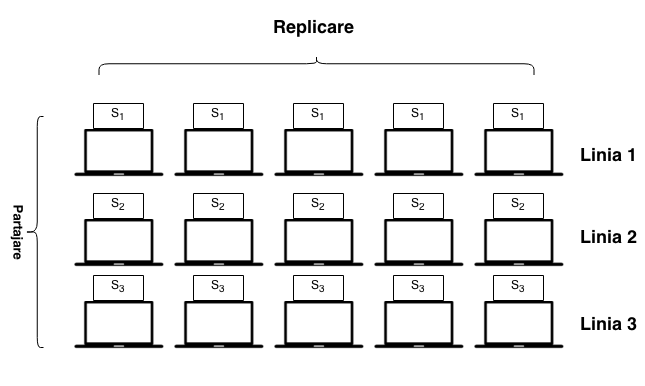
\includegraphics[width=12cm]{img/GridSharing.png}    % The printed column width is 8.4 cm.
	\caption{GridSharing cu $3$ linii, $15$ servere dintre care $2$ bizantine, $1$ cu scurgeri de informatii}
	\label{fig:grid_sharing}
	\bigskip
\end{figure}

\subsection{POTSHARDS} 
\label{sec:desc_potshards}
In 2007 este propus un nou sistem care combina caracteristicile PASIS si GridSharing adaugand posiblitatea de a k migrarea datelor la noduri noi.
De asemenea este introdusa o tehnica noua de gasire a share-urilor folosind pointeri aproximativi. Pentru a asigura confidentialitatea, autorii adopta o schema de partajare XOR te tipul totul sau nimic, la fel ca in GridSharing.
POTSHARDS readreseaza(?) problema in care o persoana neautorizata care incearca sa afle informatii vulnerabile sa nu scape nedetectata. Schemele existente precum PASIS si GridSharing nu indeplineau aceasta cerinta daca un atacator determina locatia share-urilor distribuite.

Solutia pe care o ofera PASIS este reconstruirea share-urilor insa aceasta putea sa aiba repercursiuni negative, precum dezvaluirea unor date secrete,
%maybe inserting some shard figure here
POTSHARDS poate fi gandit ca o aplicatie pe partea de client care comunica cu o multime de noduri (arhive) independente . In prima faza, POTSHARDS partajeaza obiectele in fragmente la care adauga meta-date. Autorii le numesc shard-uri. Shard-urile sunt trimise apoi arhivelor independente, fiecare avand domeniul propriu de securitate. Pentru a reconstitui cu succes obiectele, meta-datele shard-urile contin detalii despre structura pointerilor aproximativi, indicand regiunea in care se afla urmatorul shard.

Pentru un atacator, detinerea unui shard nu il ajuta foarte mult, pentru a detecta urmatorul shard, un atac brut force consta in cereri multiple in zona indicata de pointerul aproximativ. Un astfel de atac nu va trece neobservat de POTSHARDS deorece unul dintre scopurile sale este sa stocheze datele intr-un mod cat mai "imprastiat".\cite{SGMV:2009}

\section{Alouneh et al.}
\label{desc_alouneh}

Autorii propun un sistem pentru stocarea datelor un timp indelungat folosind schema Shamir cu cateva modificari. Aceste schimbari se vor arata cruciale mai tarziu in mentinerea securitatii.

\subsection{Arhitectura sistemului}
%TODO inserting figures with algoritms
In cazul in care vrem sa stocam un fisier in sistem (abordand filozofia majoritatii sistemelor de operare - orice este un fisier), acesta este preluat de o aplicatie de control pe partea de client care imparte in blocuri de octeti de lungime $k$. Pentru fiecare bloc, octetii devin coeficientii unui polinom $f$ componenta cu indicele $i$ va fi reprezentata de valoarea lui $f(i)$ $i = \{1,2,\dots, n\}$. Mentionam ca toate operatiile se vor efectua in $GF(256)$ modulo un polinom ireductibil (in implementarea sistemului, autorii folosesc $x^8 + x^5 + x^3 + x + 1$). Procedeul este descris in detaliu in Fig \ref{fig:alouneh_distribution}.


%---------------- Figure - alouneh-distribution - START ------------------------
\begin{figure*}[h!]

\begin{tabular}{|p{\textwidth}|}
\hline

\\
\hspace{.1in}
\textbf{Date de intrare}: Un fisier binar $\mathcal{S}$;
\medskip

\hspace{.1in}
\textbf{Date de iesire}: $n$ fisiere binare distribuite la noduri din retea;
\medskip

\hspace{.1in}
\textbf{Procesarea componentelor}: Aplicatia existenta pe partea clientului: 
	\begin{itemize}
		\item Daca $\mathcal{S}$ nu are o lungime divizibila cu $k$:
			\begin{itemize}
			\item concateneaza la sfarsitul lui $\mathcal{S}$ octeti pana cand $len(\mathcal{S}) \Mod k = 0$;
			\end{itemize}
		\item Imparte $\mathcal{S}$ in blocuri de lungime $k$;
		\item Repeta pentru fiecare bloc $B_t$ de lungime $k$:
		\begin{itemize}
			\item Construieste polinomul $f(x) = B_{t_{k - 1}}x ^ {k-1} + B_{t_{k - 2}}x ^ {k - 2} + .... + B_{t_1}x + B_{t_0}$;
			\item Calculeaza $f(i)$ pentru $1 \leq i \leq n$;
		\end{itemize}
	\end{itemize}

\hspace{.1in}
\textbf{Distributie}: Aplicatia la nivel de client:
	\begin{itemize}
		\item Distribuie componenta $f(i)$ nodului din retea cu indicele $i$:
	\end{itemize}

\\
\hline
\end{tabular}
\caption{Schema Alouneh et al. - Generare}
\label{fig:alouneh_distribution}
\end{figure*}

%---------------- Figure - alouneh_distribution - STOP ------------------------

\begin{example}
Vom exemplifica modul de calcul in $GF(256) \Mod {g(x)} $ unde $g(x) = x ^ 8 + x ^ 4 + x ^ 3 + 1$. Luam polinomul $f(x) = 10 + 15x$ care corespunde unui fisier format din octetii (in aceasta ordine) $10$ $15$.
	\begin{equation} \label{eq:f_01}
	\begin{split}
		f(01) \Mod{g(x)} & = 10 + 15 \Mod{g(x)} \\
		& = (x ^ 4) + (x ^ 4 + x ^ 2 + 1) \Mod{g(x)} \\
		& = x ^ 2 + 1 = 000000101_2 \\
		& =  05_{16}
	\end{split}
	\end{equation}

	\begin{equation} \label{eq:f_02}
	\begin{split}
	 f(02) \Mod{g(x)} & = 10 + 15\cdot02 \Mod{g(x)} \\
	 & = (x ^ 4) + (x ^ 5 + x ^ 3 + x) \Mod{g(x)} \\
	 & = 00111010_2 \\
	 & = 3A_{16}
	 \end{split}
	 \end{equation}
\end{example}
Pentru reconstituirea unui fisier (\ref{fig:alouneh_reconstruction}) fse interpoleaza din orice multime de componente $\mathcal{A}$ cu dimensiune minim $k$ prin metoda lui Lagrange, asemanator schemei Shamir:
\begin{equation}
	\label{eq:lagrange_poly}
	f(x)=\sum_{i \in A} f(i) \prod_{j \in A, j \neq i} \frac{x-j}{i-j}
\end{equation}

\begin{example}
Vom exemplifica interpolarea \ref{eq:lagrange_poly} pe componentele calculate in  \ref{eq:f_01} si \ref{eq:f_02} pentru a reconstitui polinomul:
	\begin{equation}
	\begin{split}
		f(x) & = 05(x - 02)(01 - 02)^{-1} + 3A(x - 01)(02 - 01)^{-1} \\
		& = 05(x - 02)03^{-1} + 3A(x - 01)03^{-1} \\
		& = F6(05 + 3A)x + F6(05\cdot02 + 3A \cdot 01) \\
		& = F6\cdot 3F\cdot x + F6\cdot30 = 15x + 10
	\end{split}
	\end{equation}
\end{example}

Noutatea arhitecturii consta in diminuarea redundantei componentelor la un factor de $k$, spre deosebire de sistemele descrise in \ref{sec:desc_pasis} sau in \ref{sec:desc_potshards}. Reducerea spatiului ocupat este datorat inlocuirii coeficientilor cu octetii din fisierul ce va fi partajat. Confidentialitatea este indusa automat de schema lui Shamir.

%---------------- Figure - alouneh-reconstruction- START ------------------------
\begin{figure*}[h!]

\begin{tabular}{|p{\textwidth}|}
\hline

\\
\hspace{.1in}
\textbf{Date de intrare}: Cel putin $k$ componente provenite din noduri (distincte);
\medskip

\hspace{.1in}
\textbf{Date de iesire}: Fisierul binar original $\mathcal{S}$;
\medskip

\hspace{.1in}
\textbf{Reconstructie}: Aplicatia existenta pe partea clientului: 
	\begin{itemize}
		\item Repeta pentru fiecare bloc al lui $\mathcal{S}$:
		\begin{itemize}
			\item Calculeaza prin interpolare coeficientii lui $f(x)=B_{t_{k - 1}}x ^ {k-1} + B_{t_{k - 2}}x ^ {k - 2} + .... + B_{t_1} + B_{t_0}$
			\item Reconstituie blocul $B_t$
		\end{itemize}
		\item Inlatura padding%(in romana?)
	\end{itemize}

\\
\hline
\end{tabular}
\caption{Schema Alouneh et al. - Reconstructie}
\label{fig:alouneh_reconstruction}
\end{figure*}

%---------------- Figure - alouneh_reconstruction- STOP ------------------------
%TODO: add reconstruction and pictures with different architectures, maybe some examples.
%----------------------------------------------------------------
%----------------------------------------------------------------
%----------------------------------------------------------------
%----------------------------------------------------------------
%----------------------------------------------------------------
\section{Rezultate obtinute}
Impreuna cu mentorul am analizat un articol aparut intr-un jurnal de clasa C unde am indentificat erori majore ale sale si am implementat sistemul descris de autori pentru a demonstra practic, nu doar teoretic anumite greseli pe care le vom evidentia in urmatoarele sectiuni. \cite{AAMK:2013}

\label{sec:results}
\subsection{Erori gasite in articol}


Spre deosebire de schema Shamir in care coeficientii sunt alesi intr-un mod aleator uniform, acestia
reprezinta acum continut din fisierele originale.
Alegerea este motivata de faptul ca multimea share-urilor si efortul computational depus pentru generarea coeficientilor se reduce la un factor de $k$ spre deosebire de schema Shamir. 
Natura determinismului duce la cateva atacuri simple in momentul in care un atacator obtine informatiile retinute intr-un nod, indiferent de marimea treshold-ului $k$.
Intuitiv, determinismul implica de cele mai multe ori vulnerabilitati (aplicarea schemei de 2 ori pe date de intrare identice $\rightarrow$ acelasi date de iesire).



\subsection{Verificarea rezultatelor}
\subsection{Publicarea articolului}

%
% ---- Bibliography ----
%
%\begin{thebibliography}{5}
%
\bibliographystyle{splncs}
\bibliography{llncs}

%\end{thebibliography}

\end{document}
